\sloppy
\documentclass[14pt,a4paper,oneside]{extarticle}	% Размер основного шрифта и формата листа
\usepackage{xltxtra}						% Используется для вывода логотипа XeLaTeX
\usepackage{xunicode}						% Кодировка документа
\usepackage{polyglossia}					% Загружает пакет многоязыковой верстки
\newfontfamily\russianfont{Book Antiqua}
%\setmainfont{Liberation Serif}						% Основной шрифт текста
\setmainfont{Book Antiqua}
\setdefaultlanguage{russian}				% Основной язык текста
\setotherlanguage{english}					% Дополнительный язык текста
\linespread{1}							% Межстрочный интервал выбран полуторным
\usepackage[left=2.5cm,
right=1.5cm,vmargin=2.5cm]{geometry} % Отступы по краям листа
\bibliographystyle{ugost2008}

\usepackage{xcolor}
\usepackage{hyperref}
% Цвета для гиперссылок
\definecolor{linkcolor}{HTML}{359B08} % цвет ссылок
\definecolor{urlcolor}{HTML}{799B03} % цвет гиперссылок
\hypersetup{pdfstartview=FitH,  linkcolor=linkcolor,urlcolor=urlcolor, colorlinks=true}

%---------------------------%
%---- Пакеты расширений ----%
%---------------------------%
\usepackage{xcolor}
\usepackage{hyperref}
% Цвета для гиперссылок
\definecolor{linkcolor}{HTML}{359B08} % цвет ссылок
\definecolor{urlcolor}{HTML}{799B03} % цвет гиперссылок
\hypersetup{pdfstartview=FitH,  linkcolor=linkcolor,urlcolor=urlcolor, colorlinks=true}


\usepackage{verbatim,indentfirst}
\usepackage{cite,enumerate,float}
\usepackage{amsmath,amssymb,amsthm,amsfonts}

%---------------------------%
%--- Вставка иллюстраций ---%
%---------------------------%
\usepackage{graphicx}
\usepackage{subfigure}
%\graphicspath{{Images/}}
\usepackage{fontspec}

\begin{document}
%	\pagestyle{empty} %  выключаенм нумерацию
%\setcounter{page}{3}% Нумерация начинается с третьей страницы
%\renewcommand{\contentsname}{\center{Содержание}}
%\tableofcontents


\begin{center}
	%\addcontentsline{toc}{section}{Опыт 11. Упругое соударение шаров}
	\subsection*{Упругое соударение шаров}
\end{center}

\begin{figure}[H]
	\centering 	
	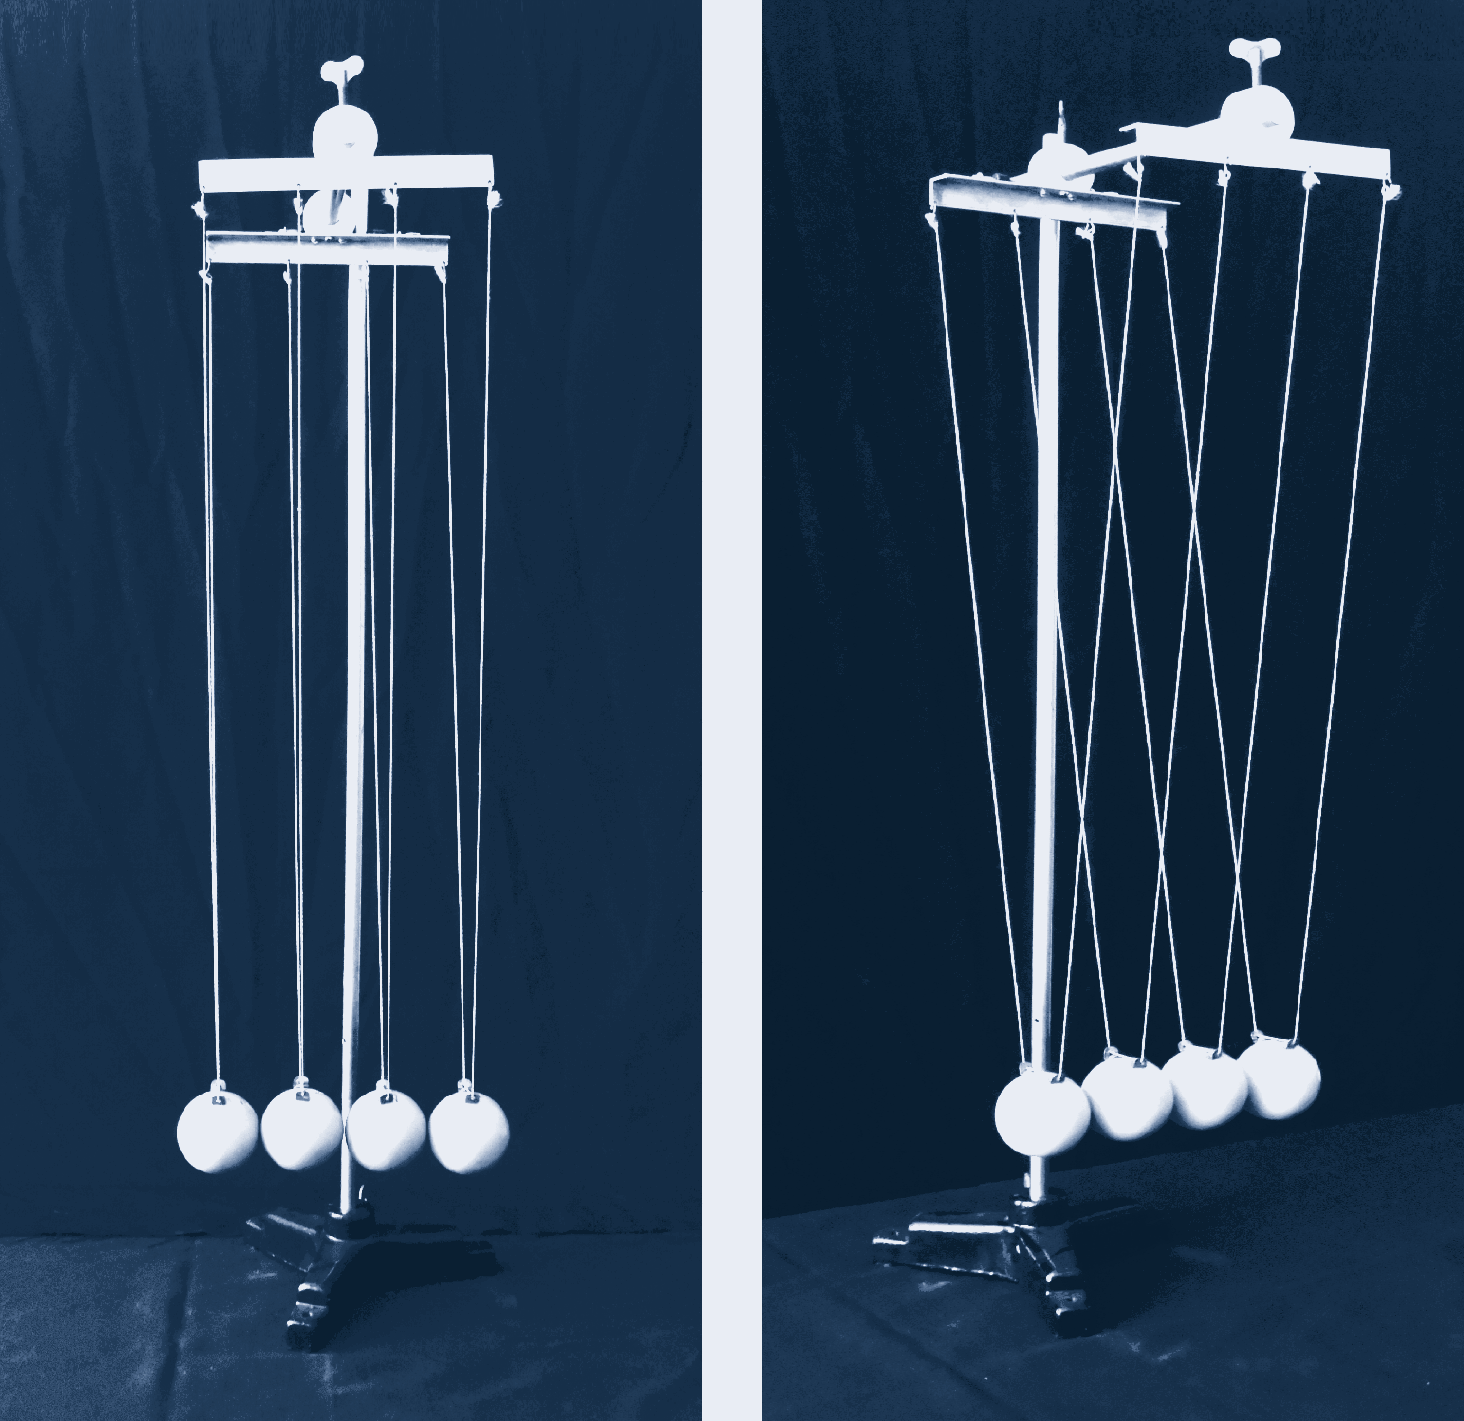
\includegraphics[width=0.75\linewidth]{impact-1.png}
	\caption{Демонстрация закона сохранения импульса при упругом ударе нескольких шаров}
	\label{impact-1}
\end{figure}

\subsection*{\underline{Оборудование:}}

\begin{enumerate}
	\item Четыре одинаковых бильярдных шара на бифилярных подвесах.
	\item Штатив.
\end{enumerate}

\subsection*{\underline{Основные определения:}}

Значение ударного импульса, появляющегося при соударении двух тел, зависит не только от их масс и скоростей до удара, но и от упругих свойств соударяющихся тел; эти свойства при ударе характеризуются величиной, называемой коэффициентом восстановления.

Величина \textit{k}, равная при прямом ударе тела о неподвижную преграду (другое тело) отношению модуля
скорости тела в конце удара к модулю скорости в начале удара, называется коэффициентом восстановления при ударе:
$$
k = \frac{v}{u}.
$$
Значение коэффициента восстановления для разных тел определяется опытным путем.

В качестве предельных случаев рассматривают случай абсолютно упругого удара ($ k=1 $), при котором кинетическая энергия тела после удара полностью восстанавливается, и случай абсолютно неупругого удара ($ k=0 $), когда вся кинетическая энергия тела теряется на его деформацию и нагревание.

\subsection*{\underline{Краткое описание:}}

Опыт, который имеет альтернативное название "Колыбель Ньютона", заключается в том, что к штативу подвешиваются четыре шара равной массы.
После этого подвес регулируется так, чтобы удар шаров был центральным (рис.\ref{impact-2}) и взаимодействие происходило попарно.
Второе условие означает, что между шарами имеется небольшой зазор, необходимый для того, чтобы после соударения один шар успевал остановиться, а другой получить и передать полученный импульс.
\begin{figure}[H]
	\centering 	
	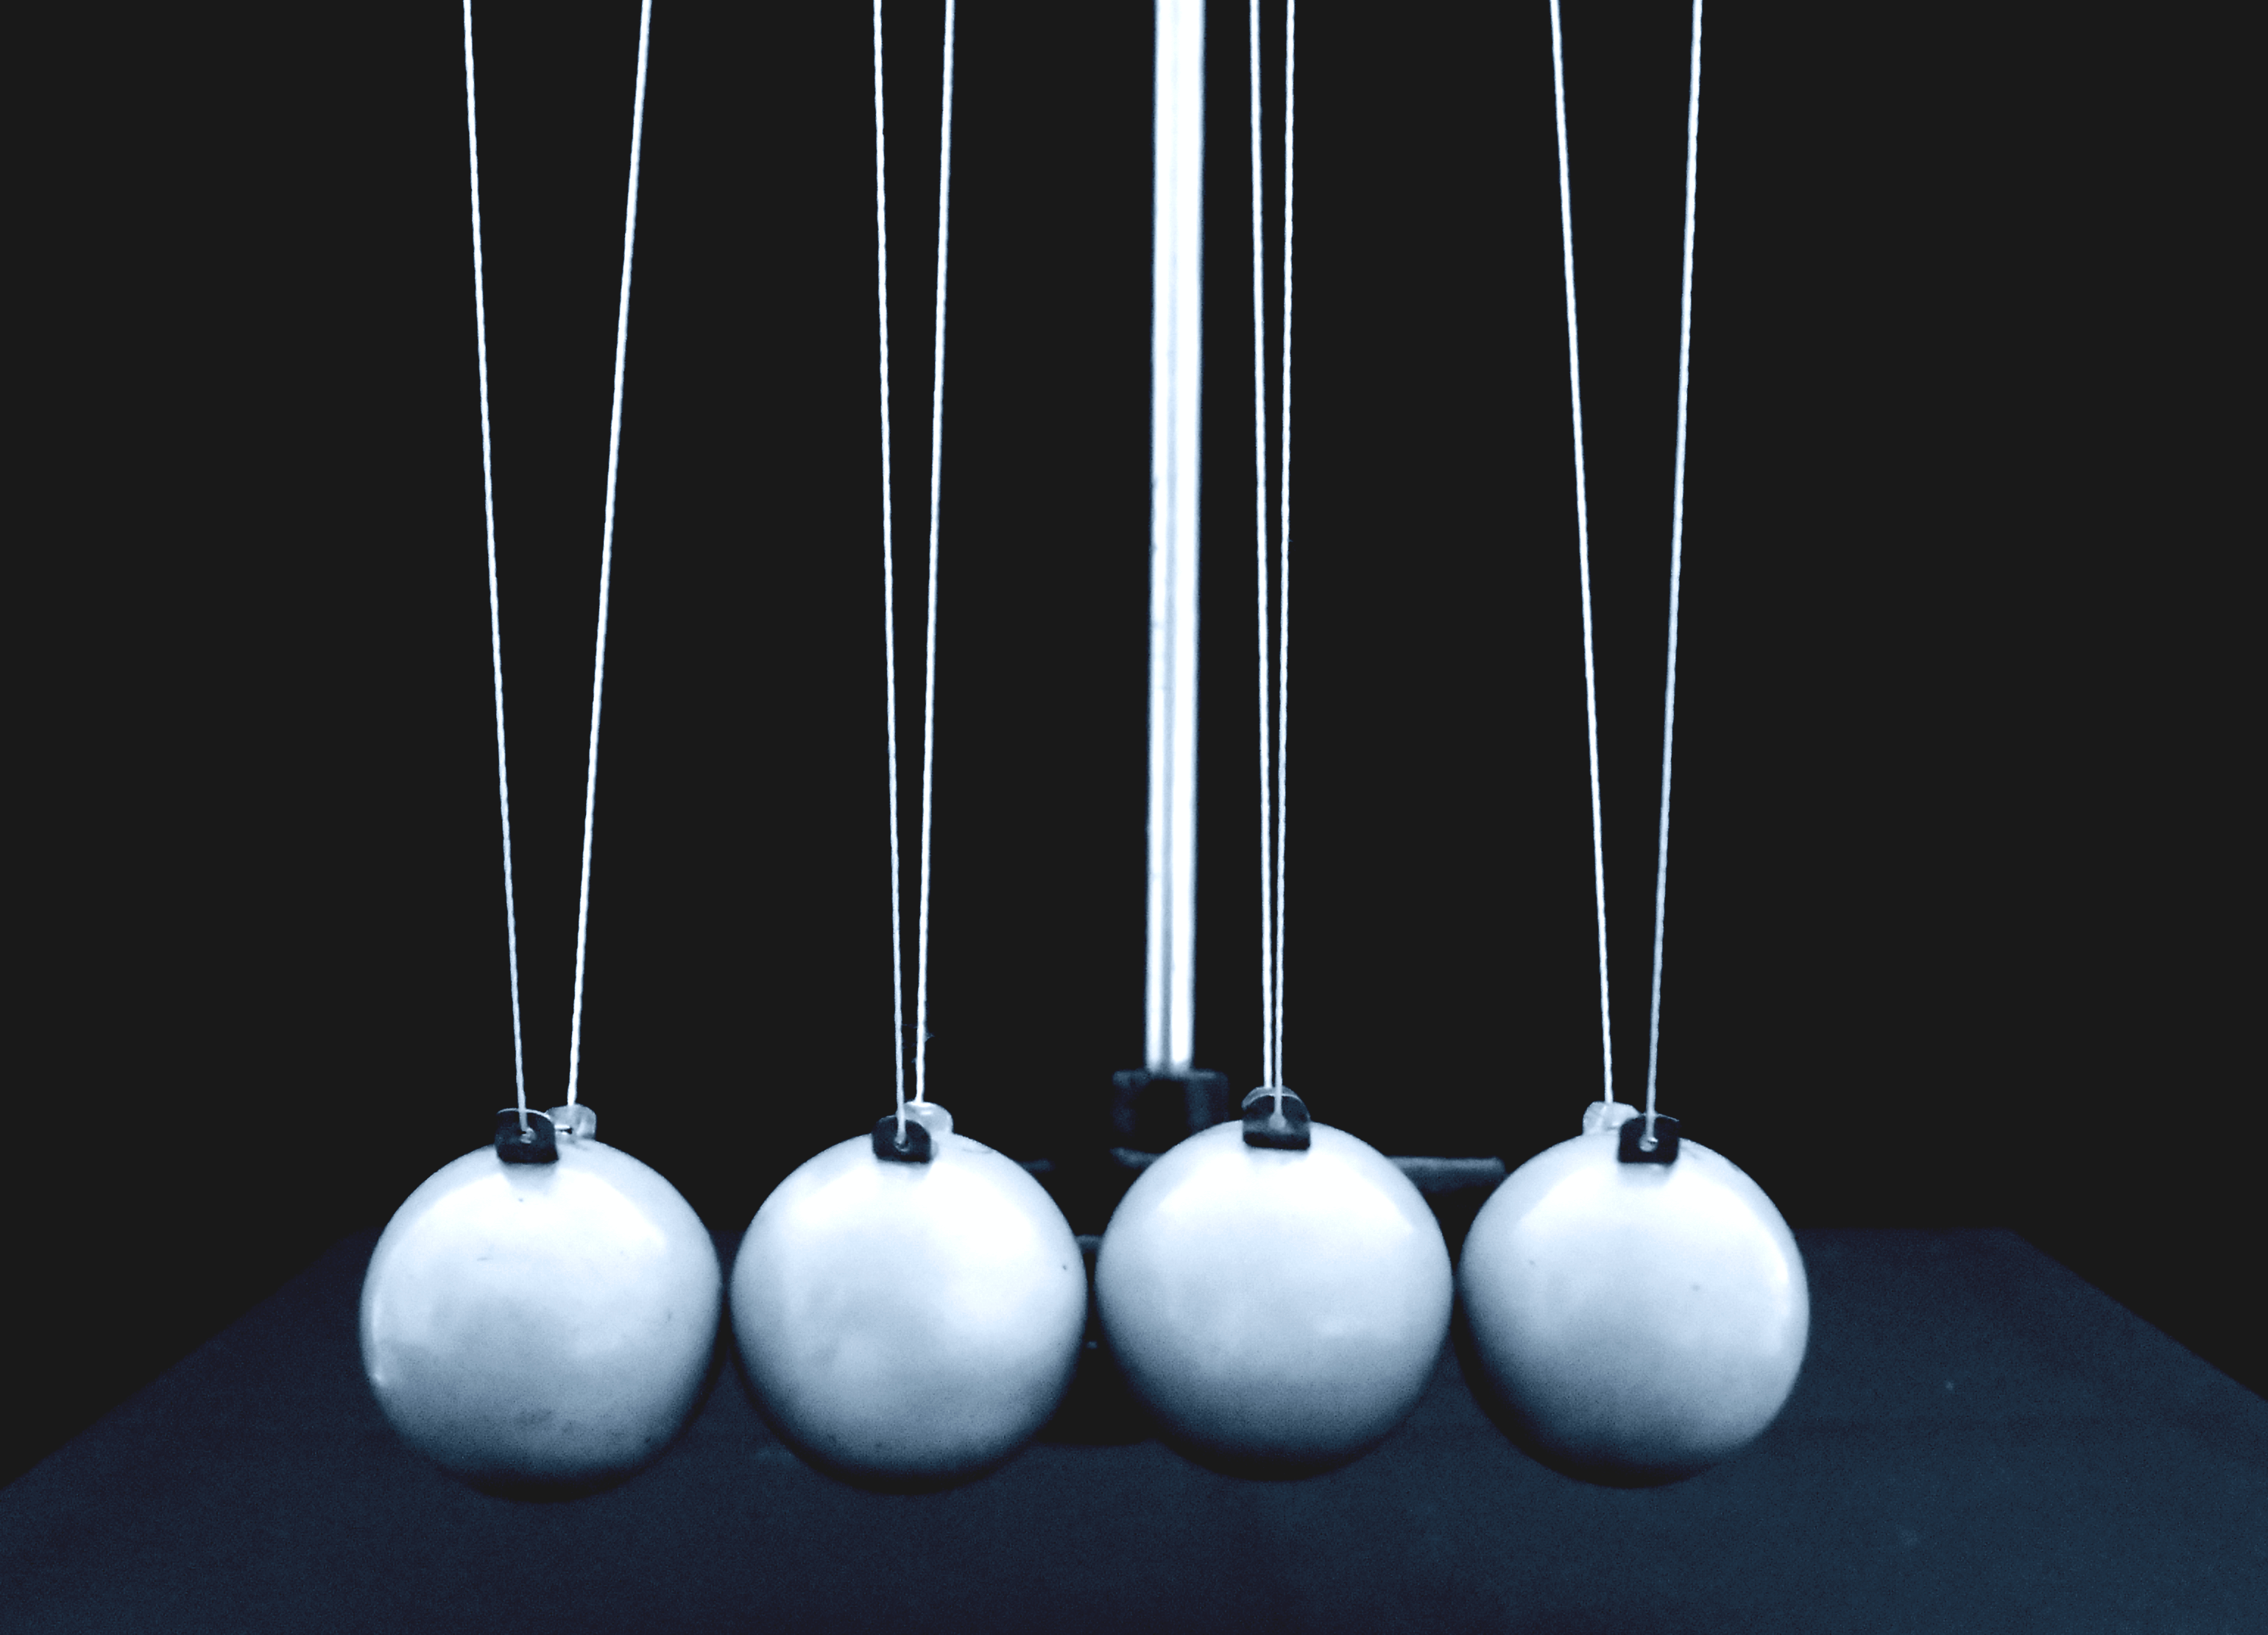
\includegraphics[width=0.6\linewidth]{impact-2.png}
	\caption{Начальное расположение шаров}
	\label{impact-2}
\end{figure}

По завершению настройки подвеса один крайний шар, подвешенный слева, отклоняется.
В этом случае после соударения и передачи импульса между шарами можно увидеть, как отскакивает шар, находящийся с правой стороны цепочки.
При этом все остальные шары, в том числе и ударяющий, остаются неподвижны (рис.\ref{impact-3}, \textit{а}).

Если отклонить два шара одновременно, то после удара от противоположного конца цепочки отскочат тоже два шара (рис.\ref{impact-3}, \textit{б}).
\begin{figure}[H]
	\centering 	
	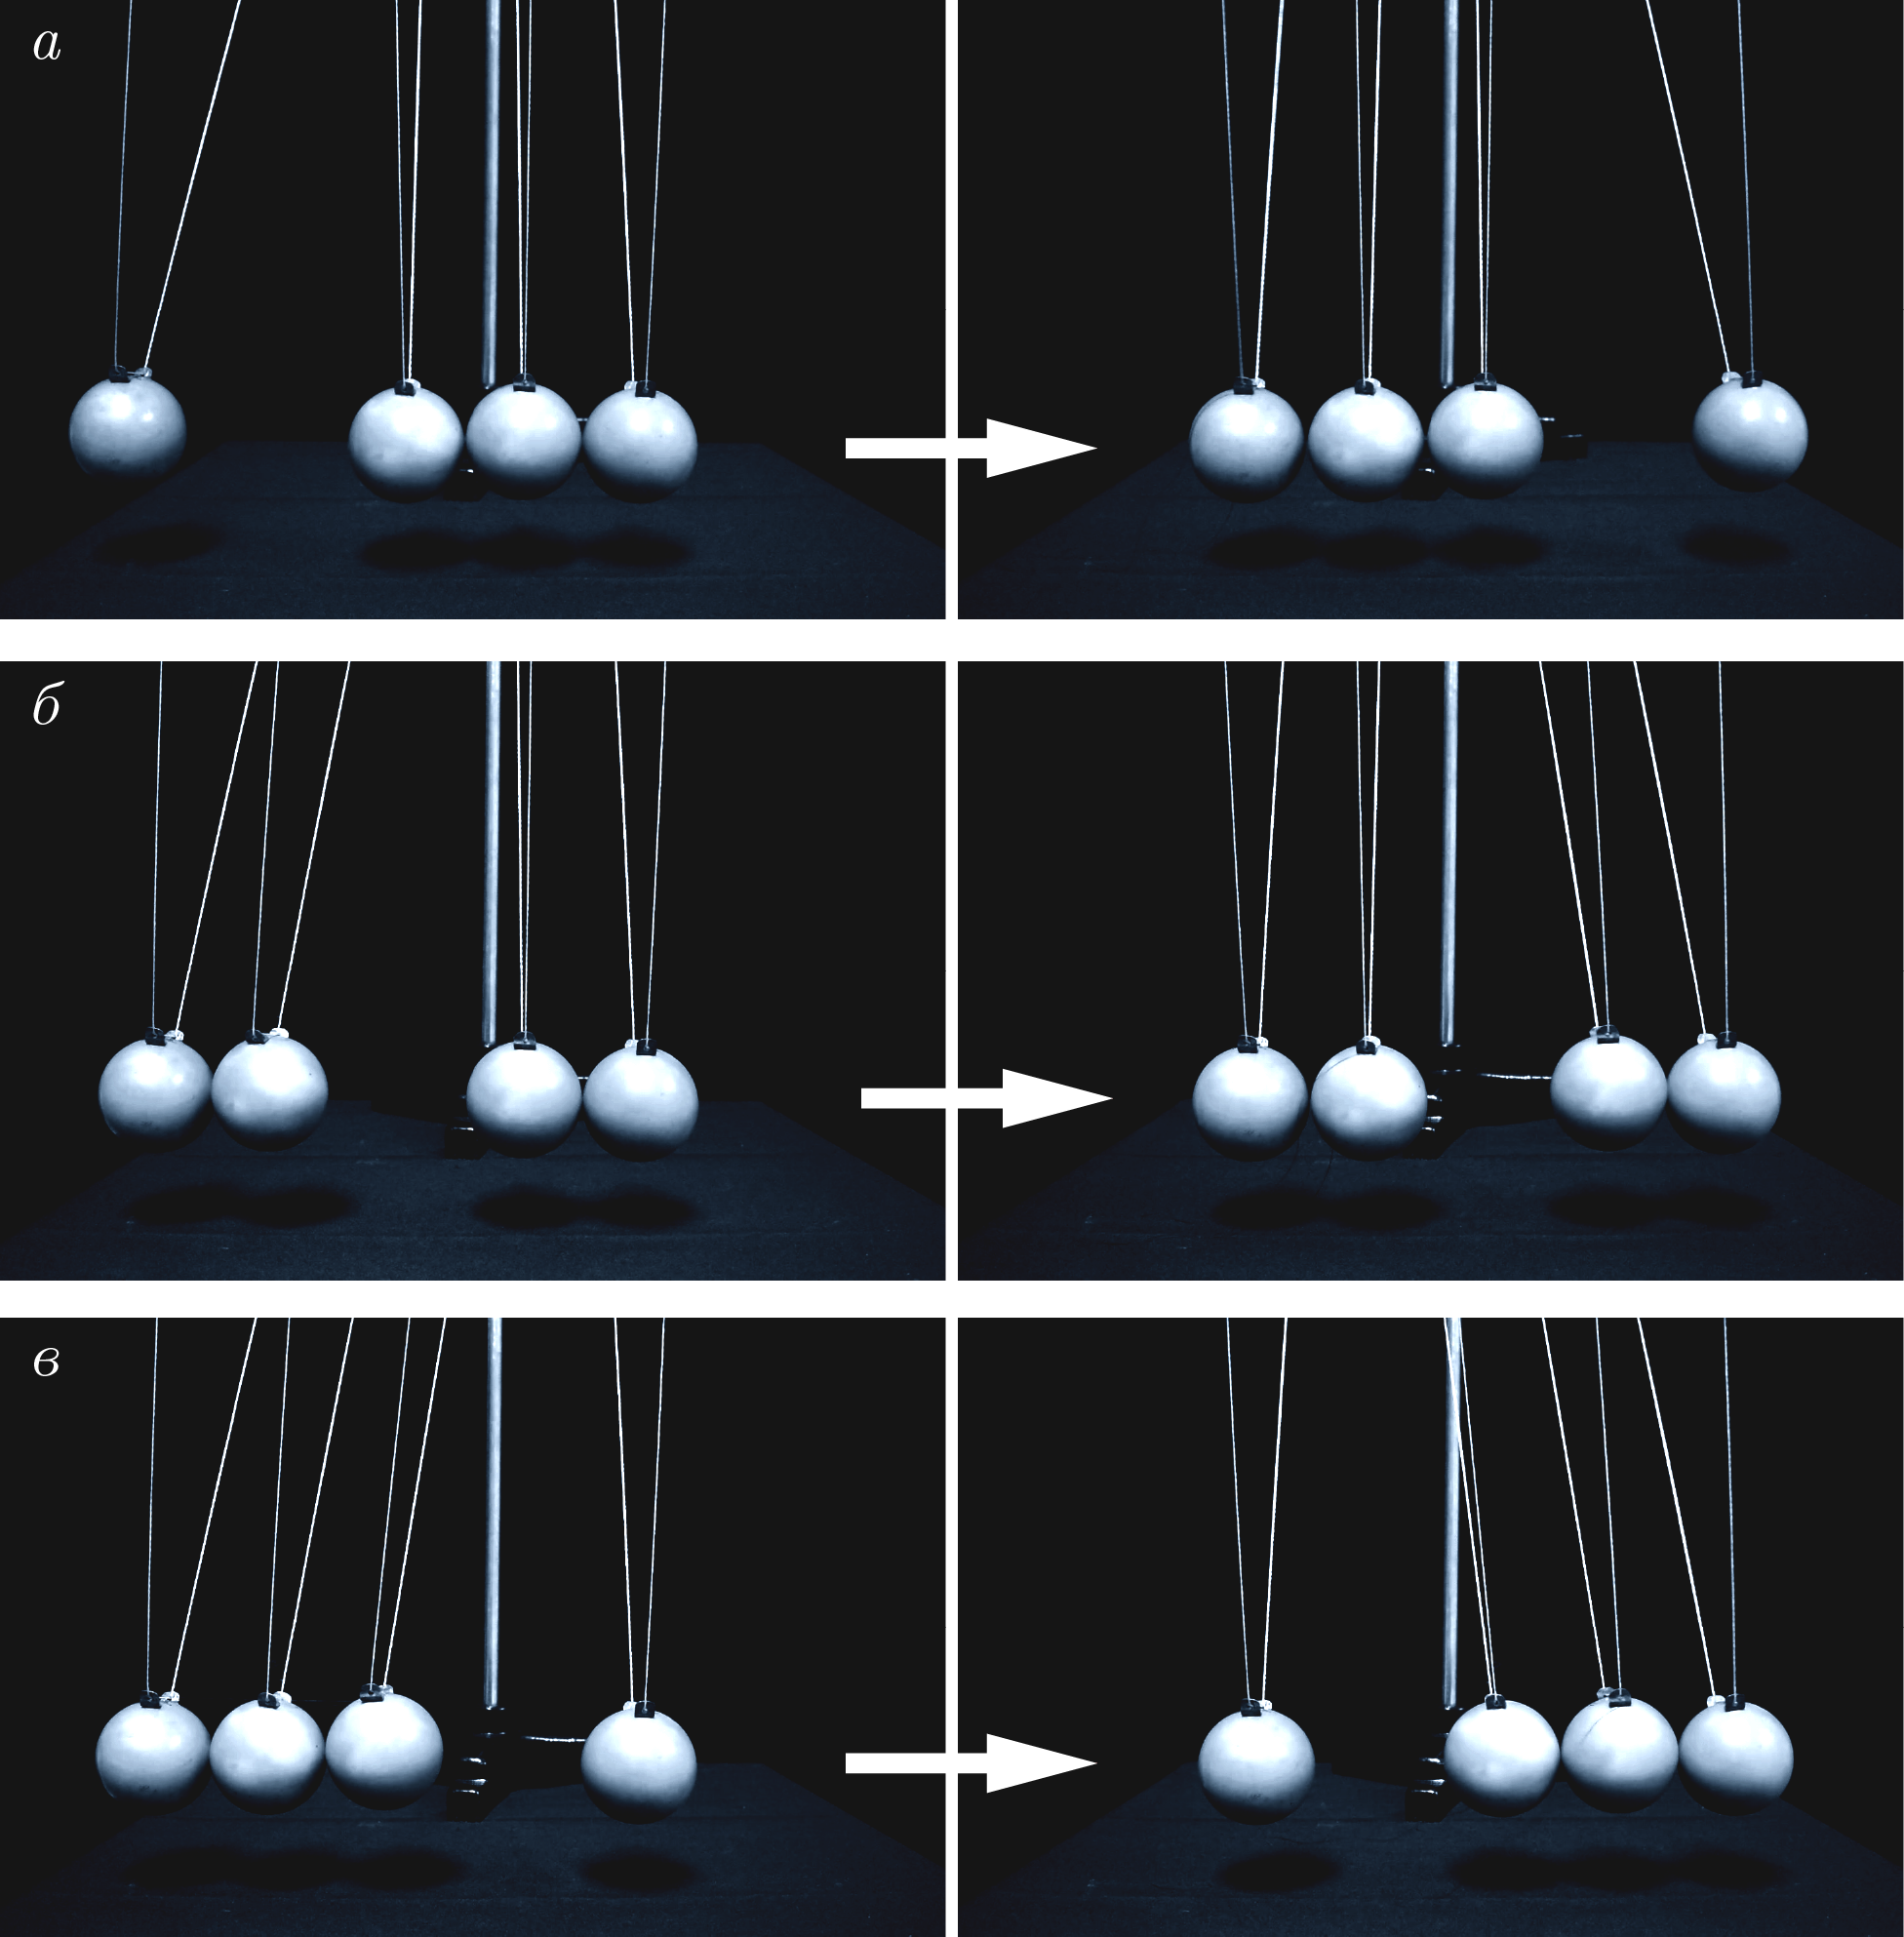
\includegraphics[width=0.9\linewidth]{impact-3.png}
	\caption{После упругого соударения отскакивает такое же число шаров (с такой же массой), которое изначально было отклонено на некоторый угол}\label{impact-3}
\end{figure}

Наконец если отклонить три соседних шара, то после удара можно наблюдать как три ударяющих шара останавливаются, зато отклоняются три шара с противоположной стороны (рис.\ref{impact-3}, \textit{в}).
При таком столкновении на месте всегда остается один шар, а отклоняется три. 

\subsection*{\underline{Теория:}}

Использование законов сохранения позволяет найти скорость движения шаров после упругого взаимодействия.
Из-за того, что в опыте количество шаров, которые в начальный момент отведены на некоторый угол, может быть различным (один, два или три шара), а массы шаров одинаковы, задачу о нахождении скорости шаров после соударения проще рассмотреть в приближении взаимодействия только двух тел:

 \begin{figure}[H]
	\centering 	
	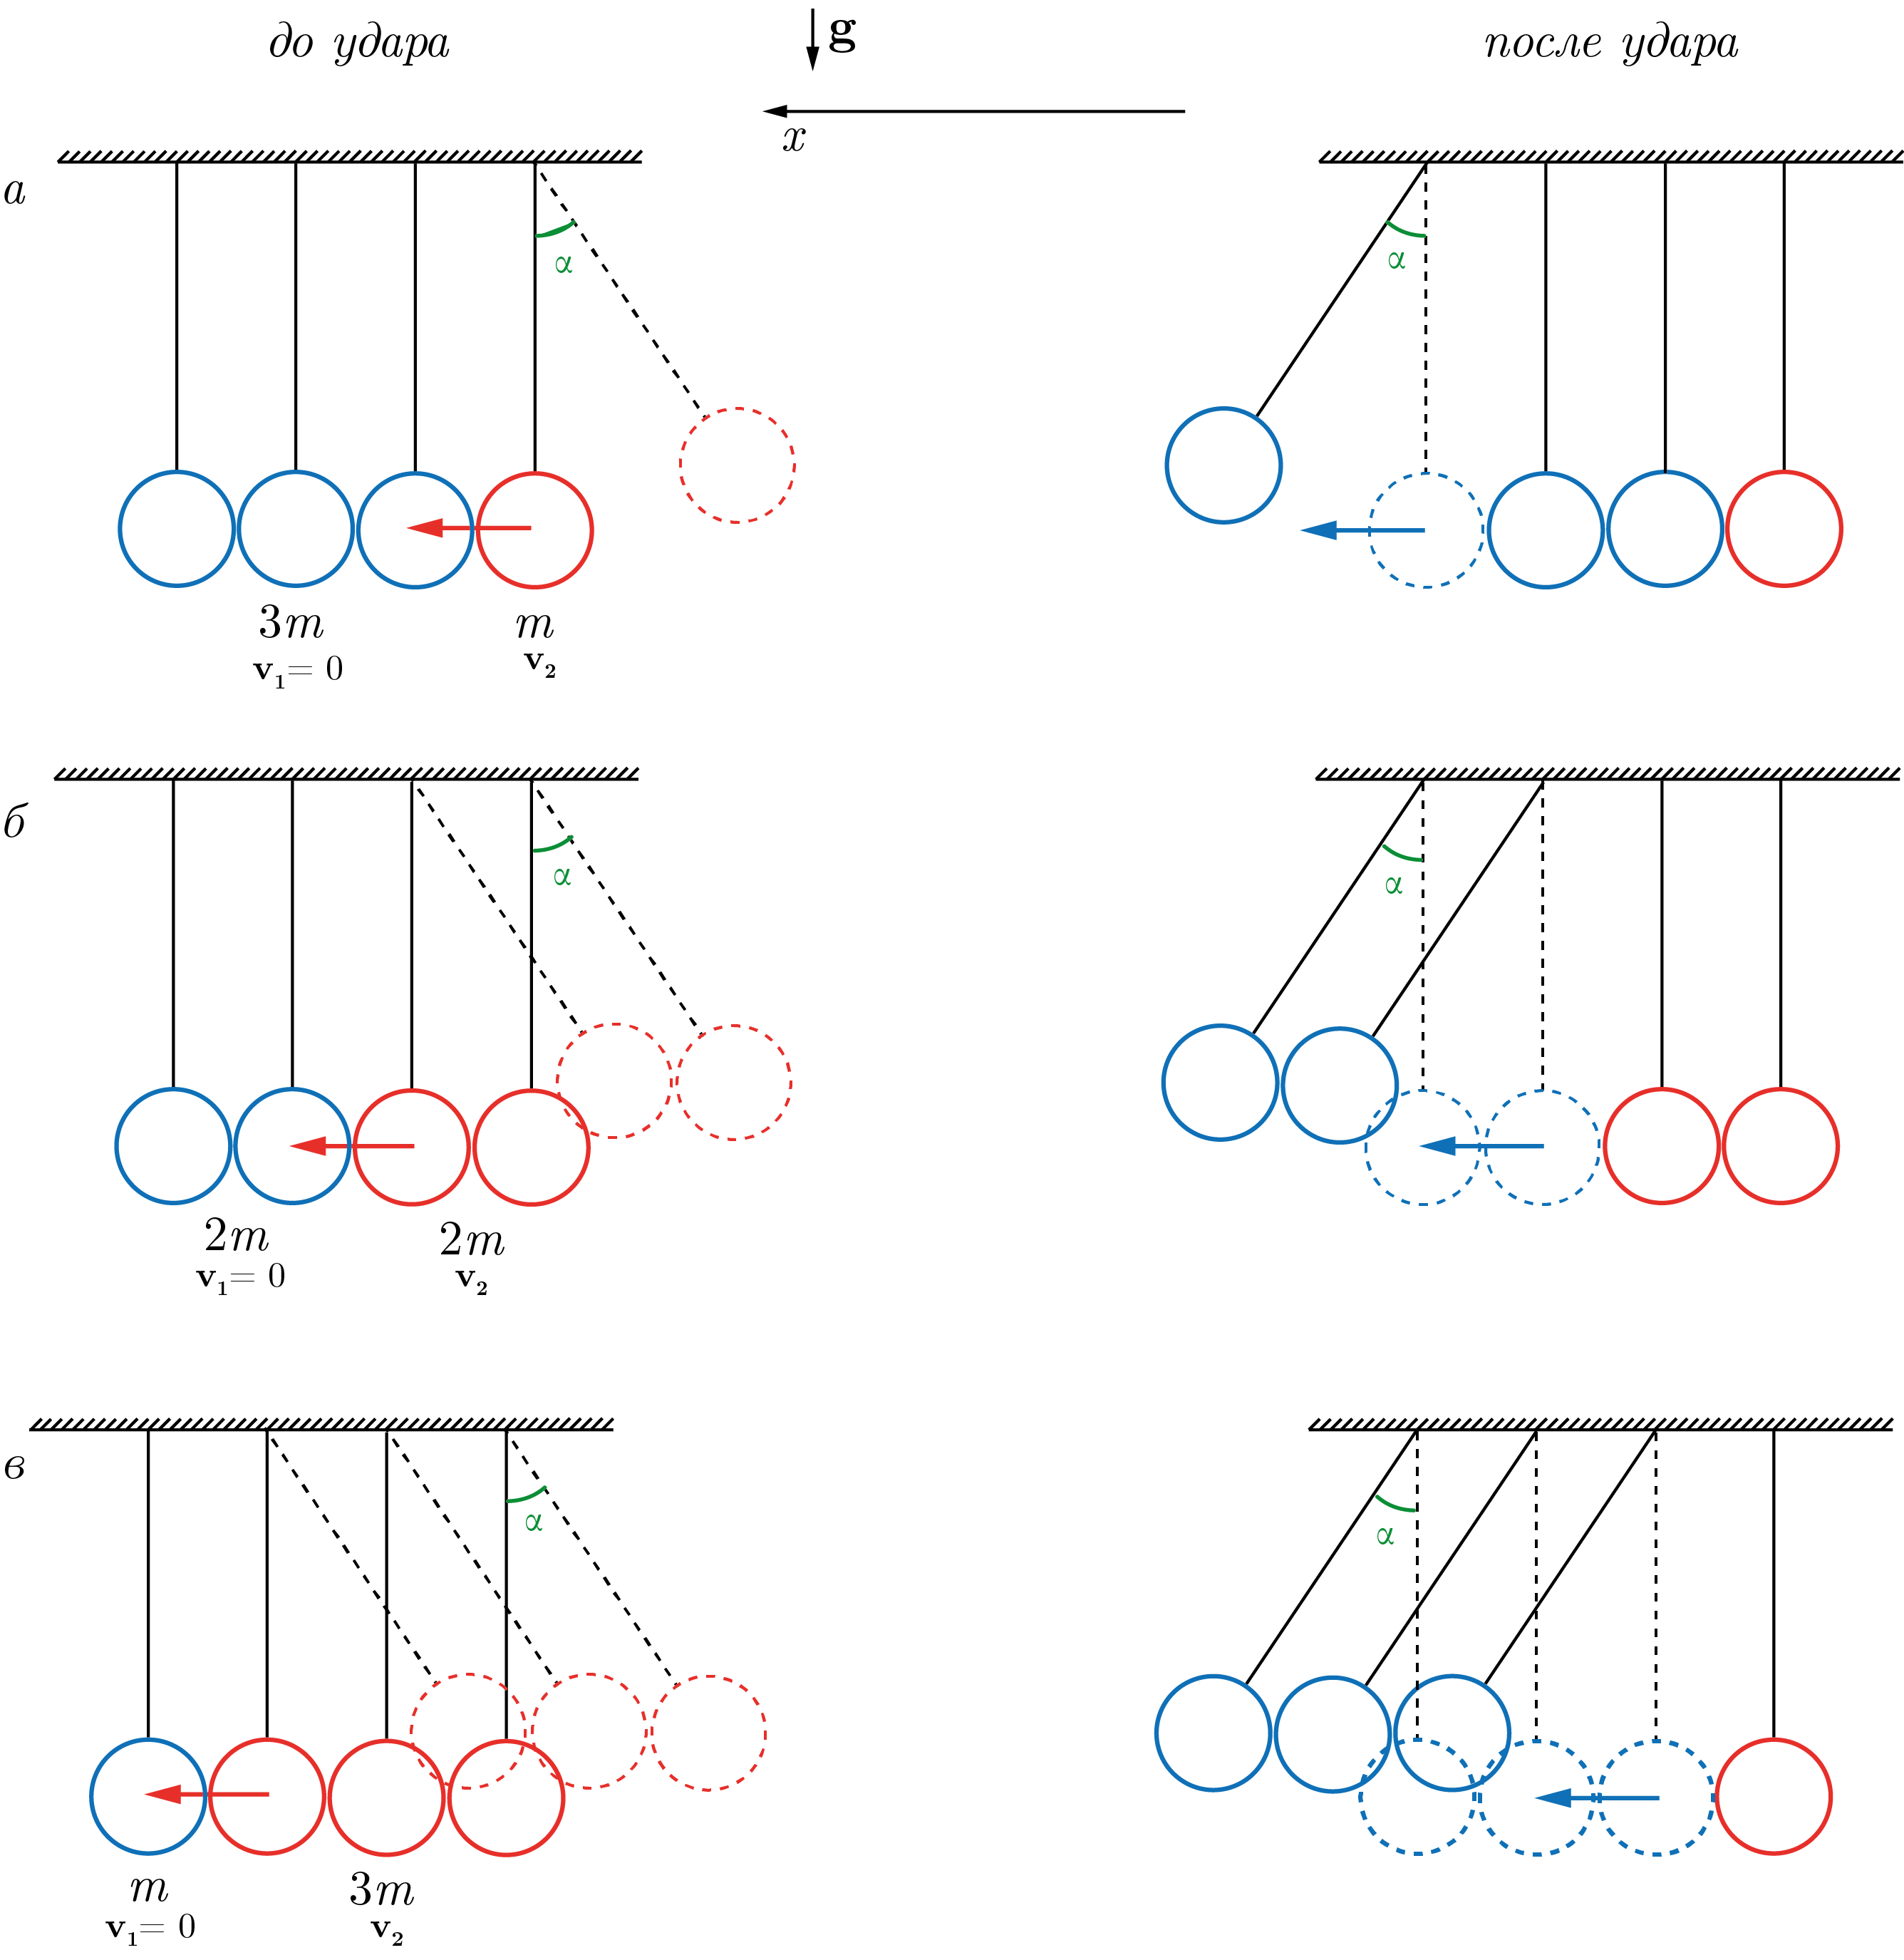
\includegraphics[width=0.8\linewidth]{impact-4.png}
	\caption{Демонстрация передачи импульса при упругом столкновении шаров одинаковой массы \textit{m}: \textit{а} — вначале на угол $ \alpha $ отклонен один шар, который при ударе передает импульс крайнему шару с противоположной стороны; \textit{б} — на угол $ \alpha $ отклонены два шара, которые после удара останавливаются, но зато на тот же угол откланяются два других шара; \textit{в} — в результате столкновения трех шаров с четвертым останавливается лишь крайний шар, причем три других шара продолжают движение в другую сторону}\label{impact-4}
\end{figure}

\begin{enumerate}
	\item отклонен один шар массой $ m_1=m $, а три других шара общей массой $ m_2=3m $ неподвижны (рис.\ref{impact-4}, \textit{а});
	\item $ m_1=m_2=2m $ — отклонены два шара  (рис.\ref{impact-4}, \textit{б});
	\item $ m_1=3m $, $ m_2=m $ — три шара сталкиваются с одним  (рис.\ref{impact-4}, \textit{в}).
\end{enumerate}

В этом случае закон сохранения проекции импульса на ось \textit{x} (индекс \textit{x} в уравнениях опущен) и энергии можно записать в виде:
\begin{equation}\label{impact-eq1}
 \begin{cases}
m_{1}v_{1} + m_{2}v_{2} = m_{1}u_{1} + m_{2}u_{2}, \\
\frac{1}{2}m_{1}v_{1}^{2} + \frac{1}{2}m_{2}v_{2}^{2} = \frac{1}{2}m_{1}u_{1}^{2} + \frac{1}{2}m_{2}u_{1}^{2},
 \end{cases}
\end{equation}
где $ v_{1} $ , $ v_{2} $ — проекции скоростей тел массами $ m_1 $ и $ m_2 $ до соударения, $ u_{1} $ и $ u_{2} $ — проекции скоростей этих тел после взаимодействия. 

Сокращая одинаковые множители во втором уравнении системы (\ref{impact-eq1}) и группируя слагаемые при $ m_1 $ и $ m_2 $, получим:
\begin{equation}\label{impact-eq2}
m_{1}(v_{1}^{2} - u_{1}^{2}) = m_{2}(u_{2}^{2} - v_{2}^{2}).
\end{equation}

Пользуясь формулой сокращенного умножения последнее уравнение можно переписать:
\begin{equation}\label{impact-eq3}
m_{1}(v_{1} - u_{1})(v_{1} + u_{1}) = m_{2}(u_{2} - v_{2})(u_{2} + v_{2}).
\end{equation}

Считая, что $ v_{1} + u_{1} = v_{2} + u_{2}  $ или $ u_{1} = v_{2} + u_{2} - v_{1} $, можно записать:
\begin{equation}\label{impact-eq4}
m_{1}(v_{1} - u_{1}) = m_{2}(u_{2} - v_{2}).
\end{equation}
Тогда уравнение (\ref{impact-eq3}) примет следующий вид:
\begin{equation}\label{impact-eq5}
m_{1}v_{1} + m_{2}v_{2} = m_{1}u_{2} + m_{1} (v_{2} + v_{1}) + m_{2}u_{2},
\end{equation}
или
\begin{equation}\label{impact-eq6}
u_{2} (m_{1}+m_{2}) = 2m_{1}v_{1} + (m_{2}-m_{1})v_{2}.
\end{equation}

В итоге для скорости второго (отскочившего) шара $ m_{2} $ после соударения получим выражение:
\begin{equation}\label{impact-eq7}
u_{2} = \frac{ 2m_{1}v_{1} + (m_{2}-m_{1})v_{2}}{m_{1}+m_{2}}
\end{equation}
или
\begin{equation}\label{impact-eq8}
u_{2} = v_{2} + \frac{ 2m_{1}}{m_{1}+m_{2}} (v_{1}-v_{2}).
\end{equation}

Для первого шара $ m_{1} $ скорость после соударения можно рассчитать по формуле:
\begin{equation}\label{impact-eq9}
u_{1} = v_{1} - \frac{ 2m_{2}}{m_{1}+m_{2}} (v_{1}-v_{2}).
\end{equation}

В частном случае, если сталкиваются одинаковые тела ($ m_{2}=m_{1} $, причем одно из них в момент абсолютно упругого удара покоится ($ v_{2}=0 $), то скорость этого тела после взаимодействия с телом той же массы станет равна скорости движущегося тела, $ u_{2}=v_{1} $.
При этом тот шар, который сталкивается с изначально неподвижным телом, остановится, а его импульс передастся второму шару, который отклонится на тот же угол, что и первый.

\end{document}